\chapter{Performance experiments}

The performance experiments were designed to explore the parallel performance of ABC SMC inference framework which were used in the parameter estimation and model selection tasks. Usually ABC SMC is a time-consuming and computation intensive task and ideally executed on large clusters. The scheduling strategy, implementation details and many other factors can affect the parallel efficiency.

    [MORE meanings of the performance study]

\section{Scaling-up}

First experiments are designed to illustrate the scaling-up performance. The program used here is an implementation of ABc SMC on model 5. The details of the ABC SMC settings is listed below

\begin{itemize}
    \item Prior distribution: default to log-uniform distribution [$1\times 10^{-6}$, 50] for all the 12 parameters
    \item threshold schedule: median epsilon
    \item No factors, no adaptive distance or adaptive population applied
    \item Population size is 2000, with 20 generations
\end{itemize}

[HOW PYABC parallelise the sampling]

For HPC systems like Cirrus, \verb|pyabc| uses \verb|multiprocessing| for multi-core parallel sampling. By default if the number of cores is not specified, it will automatically read the number of available cores and use them all. Cirrus has a 36-core CPU which support hyperthreading, such that the maximal number of cores available to \verb|multiprocessing| is 72.

The program is executed on Cirrus, using 8, 16, 24, 36, 54 and 72 cores respectively. Each run is repeated 10 times. The average execution time, required sampling numbers are recorded. Hyperthreading is enabled when using 54 and 72 cores. The access to the node that contains computation cores is exclusive, such that the execution would not be affected by other programs of operations.

The implementation of ABC SMC in \verb|pyabc| enables the parallelisation of sampling, which is the must time-consuming part. The rest part of the program is mostly not parallelised, e.g. database I/O and reductions operations. The sampling process involves sampling, perturbation and test of the acceptance criteria, all of which are computation-intensive.

In practice, using ABC SMC to estimate the parameters of a given model could cost up to several hundred of hours if the computational resources is limited[REF]. The performance experiment result could provide a reference that illustrate that how the efficiency changes when scaling-up or the trade-offs in computational resources' cost and their benefit.

\subsubsection{Results}

[scaling-up performance: speed-up and efficiency]

[large variation in required sampling numbers]

[possible reasons]

\begin{figure}[h]
    \begin{center}
        \resizebox{1.0\hsize}{!}{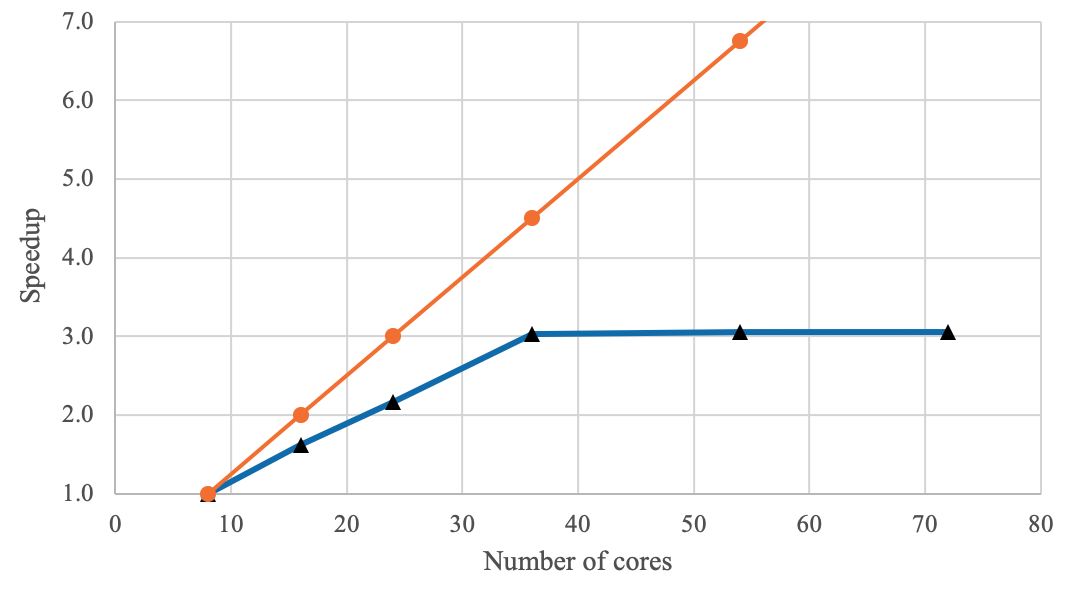
\includegraphics{fig/speedup.png}}
    \end{center}

    \caption[TODO]{Speedup. MORE DESCRIPTION}
    \label{fig:speedup}
\end{figure}

The recorded execution time using different number of cores is shown in FIGURE. According to that, speed-up and efficiency can be calculated. Here 8 cores is regarded as the baseline for speed-up and efficiency, as the serial version (using only one core) can take quite a long time to finish 10 repeats. When increasing number of cores, the execution time drops fast at first but the decreasing rate (dropping speed, i.e. the derivative of the execution time against time) is gradually reduced to zero; 36, 54 and 72 cores gives nearly the same average execution time and consequently gains very close speedup values (FIGURE).

Denote the number of cores used in the ABC SMC runs as variable $p$. The speedup curve shows a linear trend when $p\leq 36$; when $p\geq 36$ the speedup stays nearly unchanged. $p=36$ is an inflection point, where 36 is the maximum numbers available physical cores in a compute node of Cirrus. A constant drop of efficiency is observed when increasing $p$; smaller $p$ ($p<36$) gives an efficiency higher than 65\% but greater $p$ e.g. $p=72$ results in a low efficiency (34\%).

\begin{figure}[h]
    \begin{center}
        \resizebox{1.0\hsize}{!}{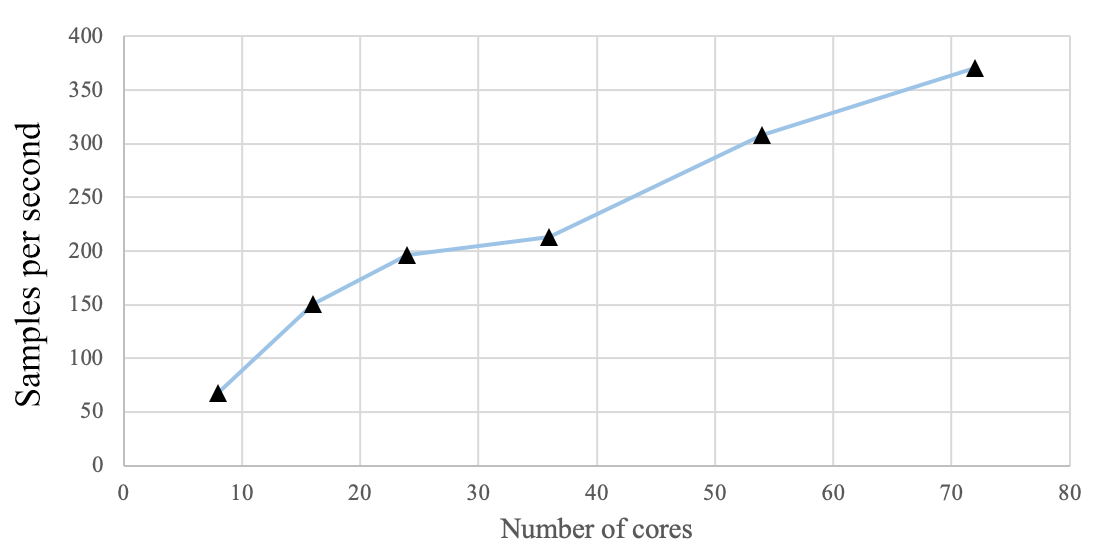
\includegraphics{fig/sample_per_time.png}}
    \end{center}

    \caption[TODO]{Samples per second. MORE DESCRIPTION}
    \label{fig:sample_per_sec}
\end{figure}

A high variance of total required samples was observed in the scaling-up experiments: some single runs required much more samples to finish 20 populations. Moreover, we found that the execution time is not ideally proportional to the total required samples (FIGURE). A possible explain to these phenomenons can be that the median epsilon schedule results in different threshold strategies due to the randomness in the sampling process, thus results in different approximate convergency paths for different runs. Some runs that are stuck in a local optimum and require smaller target epsilon will take huge amount of samples to move away from the local optimum. This have been observed when the distribution of posterior is plotted before and after jumping away from local modes (FIGURE and more explain). Also, time spent in each sample using sanme number of cores is not constant in our case, which might be a result of the parallel schedule; ideally a serial run using only one core will see a nearly constant time spent in every particle.

Due to the unstable sampling numbers, our interests switched to the per-particle performance, where the average sampling numbers per second (FIGURE) and average time spent in one particle (FIGURE) under different of cores ($p$) are plotted. The log-like average time per particle curve shows that using more cores can improve the sampling efficiency, but when $p$ is at a high level (e.g. 36 in our case), the improvement will be less significant.

\section{Profiling}

The performance could also be analysed given a profiling report. The second experiment profiles the program to reveal the detailed time consumption for each operation and the possible bottleneck, according to which we could find the hot-spot of program and given possible suggestions on improving the performance.

In this case, profile tools \verb|cProfile| and \verb|yappi| is used in PyCharm IDE.

\subsubsection{Results}

[profiling results: hot-spot and possible improvements]
